\documentclass[a4paper, 12pt, twoside]{article}
\usepackage[T2A,T1]{fontenc}
\usepackage[utf8]{inputenc}
\usepackage[english, russian]{babel}
\usepackage{graphicx}
\usepackage[hcentering, bindingoffset = 10mm, right = 15 mm, left = 15 mm, top=20mm, bottom = 20 mm]{geometry}
\usepackage{multirow}
\usepackage{ gensymb }
\usepackage{lipsum}
\usepackage{amsmath, amstext}
\usepackage{siunitx}
\usepackage{subcaption}
\usepackage{wrapfig}
\usepackage{adjustbox}
\usepackage{enumerate, indentfirst, float}
\usepackage{capt-of, svg}
\usepackage{ctable}

\newcommand*{\hm}[1]{#1\nobreak\discretionary{} 
	{\hbox{$\mathsurround=0pt #1$}}{}}
\usepackage{cmap} % Улучшенный поиск русских слов в полученном pdf-файле

\usepackage{pscyr} % Нормальные шрифты
\usepackage[normalem]{ulem} % для подчёркиваний uline
\ULdepth = 0.16em

\usepackage{fancyhdr} %Колонтикулы
\pagestyle{fancy}
\lhead{
\includegraphics[width = 10 mm]{logo.jpg} Лабораторная работа № 4.7.3}
\rhead{\textit{31 марта 2018 г.}}

\newenvironment{bottompar}{\par\vspace*{\fill}}{\clearpage}

\begin{document}
	\begin{titlepage}
		
		\newcommand{\HRule}{\rule{\linewidth}{0.7mm}} % Defines a new command for the horizontal lines, change thickness here
		
		\center % Center everything on the page
		
		%----------------------------------------------------------------------------------------
		%	HEADING SECTIONS
		%----------------------------------------------------------------------------------------
		
		\textsc{\LARGE Московский Физико-Технический Институт}\\[1,5cm] % Name of your university/college
		\textsc{\Large Кафедра общей физики}\\[0.5cm] % Major heading such as course name
		\textsc{\large Лабораторная работа \textnumero  4.7.3}\\[0.5cm] % Minor heading such as course title
		
		%----------------------------------------------------------------------------------------
		%	TITLE SECTION
		%----------------------------------------------------------------------------------------
		
		\HRule
		\\[0.4cm]
		{ \huge \bfseries Изучение поляризованного света.}
		\\[0.2cm] % Title of your document
		\HRule
		\\[1.5cm]
		
		
		
		%----------------------------------------------------------------------------------------
		%	AUTHOR SECTION
		%----------------------------------------------------------------------------------------
		
		\begin{minipage}{0.4\textwidth}
			\begin{flushleft} \large
				\textbf{Автор:}\\
				Глеб Уваркин \\
				615 группа
			\end{flushleft}
		\end{minipage}
		~
		\begin{minipage}{0.4\textwidth}
			\begin{flushright} \large
				\textbf {Преподаватель:} \\
				Клёнов Сергей Львович % Supervisor's Name
			\end{flushright}
		\end{minipage}
		
		\begin{bottompar}
			\begin{center}
				
\includegraphics[width = 80 mm]{logo.jpg}
			\end{center}
			{\large 31 марта 2018 г.}
			
		\end{bottompar}
		\vfill % Fill the rest of the page with whitespace
		
	\end{titlepage}
	
	{\Large \uline { \textbf  {Цель работы:}}}
	
	\vspace{2mm}
	Ознакомление с методами получения и анализа поляризованного света.

	\vspace{\baselineskip}
	
	{\Large \uline { \textbf  {В работе используются:}}}
	
	\vspace{2mm}
	
	Оптическая скамья с осветителем; зеленый светофильтр; два поляроида; черное зеркало; полированная эбонитовая пластинка; стопа стеклянных пластинок; слюдяные пластинки разной толщины; пластинки в 1/4 и 1/2 длины волны; пластинка в одну длину волны для зеленого света (пластинка чувствительного оттенка).
	
	\section{Теоретические сведения.}
	
	\paragraph{Естественный и поляризованный свет.} 
	
	Как известно, световые волны поперечны: электрический вектор $\mathbf{E}$ и магнитный вектор $\mathbf{H}$ (или $\mathbf{B}$) взаимно перпендикулярны и располагаются в плоскости, перпендикулярной направлению распространения волны (лучу $\mathbf{S}$). Во всякой данной точке пространства ориентация пары векторов $\mathbf{E}$ и $\mathbf{H}$ в плоскости, перпендикулярной лучу $\mathbf{S}$, может, вообще говоря, изменяться со временем. В зависимости от характера такого изменения различают естественный и поляризованный свет.
	
	Обычные источники света являются совокупностью огромного числа быстро высвечивающихся ($10^{-10} \div 10^{-9}$) элементарных источников (атомов или молекул), испускающих свет независимо друг от друга, с разными фазами и с разными ориентациями векторов $\mathbf{E}$ и $\mathbf{H}$. Ориентация векторов $\mathbf{E}$ и $\mathbf{H}$ в результирующей волне поэтому хаотически изменяется во времени, так что в плоскости, перпендикулярной лучу $\mathbf{S}$, все направления оказываются в среднем равноправными. Такой свет называют естественным или неполяризованным.
	
	При помощи специальных приспособлений (поляризаторов) естественный свет может быть превращен в линейно поляризованный. В линейно поляризованной световой волне пара векторов $\mathbf{E}$ и $\mathbf{H}$ не изменяет с течением времени своей ориентации. Плоскость $\mathbf{E}$, $\mathbf{S}$ называется в этом случае плоскостью колебаний.
	Наиболее общим типом поляризации является эллиптическая поляризация. В эллиптически поляризованной световой волне конец вектора	$\mathbf{E}$ (в данной точке пространства) описывает некоторый эллипс. Линейно поляризованный свет можно рассматривать как частный случай эллиптически поляризованного света, когда эллипс поляризации вырождается в отрезок прямой линии; другим частным случаем является круговая поляризация (эллипс поляризации является окружностью).\\
	
	\begin{minipage}{0.6 \linewidth}
		При теоретическом рассмотрении различных типов поляризации часто бывает удобно проектировать вектор E в некоторой точке пространства на два взаимно перпендикулярных направления (рис. 1). В том случае, когда исходная волна была поляризованной, Ex и Ey когерентны между собой и могут быть записаны в виде
		\begin{equation}
		E_x = E_{x_0} \cos (kz - \omega t),
		~
		E_y = E_{y_0} \cos (kz - \omega t - \varphi)
		\end{equation}
		
		где амплитуды $E_{x_0}$, $E_{y_0}$, волновой вектор k, частота $\omega$ и сдвиг фаз $\varphi$ не зависят от времени. Формулы (1) описывают монохроматический свет. Немонохроматический свет может быть представлен суммой выражений типа (1) с различными значениями частоты $\omega$. 
	\end{minipage}
	~
	\begin{minipage}{0.39\linewidth}
		\begin{figure}[H]
			\centering
			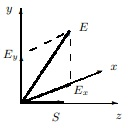
\includegraphics[width =  0.6\textwidth]{ris1}
			\caption{Представление световой волны в виде двух линейно поляризованных волн.}
			\label{ris1}
		\end{figure}
	\end{minipage}\\
	
	
	Ориентация эллипса поляризации определяется отношением амплитуд $E_{y_0}/E_{x_0}$ и разностью фаз $\varphi$. В частности, при $\varphi = 0, \pm \pi$ эллипс вырождается в отрезок прямой (линейная поляризация). При $\varphi = \pm \varphi \pi/2$ главные оси эллипса совпадают с осями x, y. Если при этом отношение амплитуд $E_{y_0}/E_{x_0} = 1$, эллипс поляризации вырождается в окружность 2.
	
	В плоскости $z = z_0$ вектор $\mathbf{E}$ волны (1) вращается против часовой стрелки (при наблюдении навстречу волне), если $0 < \varphi < \pi$. В этом	случае говорят о левой эллиптической поляризации волны. Если же $\pi < \varphi < 2\pi$, вращение вектора $\mathbf{E}$ происходит по часовой стрелке, и волна имеет правую эллиптическую поляризацию.
	
	В фиксированный момент времени $t = t_0$ концы вектора $\mathbf{E}$ при различных z лежат на винтовой линии. При этом для левой эллиптической поляризации образуется левый винт, а для правой -- правый винт.
	
	Неполяризованный свет также может быть разложен на две линейно поляризованные компоненты; однако в этом случае разность фаз $\varphi$ испытывает быстрые хаотические изменения, так что колебания $E_x$ и $E_y$ оказываются некогерентными.
	
	\paragraph{Методы получения линейно поляризованного света.}
	
	Для получения линейно поляризованного света применяются специальные оптические приспособления — поляризаторы. Направление колебаний электрического вектора в волне, прошедшей через поляризатор, называется	разрешенным направлением поляризатора.
	
	Всякий поляризатор может быть использован для исследования поляризованного света, т. е. в качестве анализатора. Интенсивность I линейно поляризованного света после прохождения через анализатор зависит от угла, образованного плоскостью колебаний с разрешенным направлением анализатора:
	\begin{equation}
	I = I_0 \cos^2 \alpha 
	\end{equation}
	
	Соотношение (2) носит название закона Малюса.\\
	
	\textit{\textbf{Отражение света от диэлектрической пластинки.}} Отраженный от диэлектрика свет всегда частично поляризован. Степень поляризации света, отраженного от диэлектрической пластинки в воздух, зависит от показателя преломления диэлектрика $n$ и от угла падения $i$. Как следует из формул Френеля, полная поляризация отраженного света достигается
	при падении под углом Брюстера, который определяется соотношением
	\begin{equation}
	\tg i = n 
	\end{equation}
	
	В этом случае плоскость колебаний электрического вектора в отраженном свете перпендикулярна плоскости падения.
	
	\paragraph{Получение эллиптически поляризованного света.} 
	Эллиптически поляризованный свет можно получить из линейно поляризованного с
	помощью двоякопреломляющих кристаллических пластинок. Двоякопреломляющая пластинка имеет два взаимно перпендикулярных главных направления, совпадающих с осями эллипсоида диэлектрической проницаемости. Волны, поляризованные вдоль главных направлений, распространяются в пластинке с разными скоростями, не изменяя
	характера своей поляризации. Эти волны называются главными.	Мы будем обозначать показатели преломления для главных волн через $\eta_\xi$ и $\eta_\eta$, где $\xi$ и $\eta$ -- главные направления кристаллической пластинки	(рис. 2).\\

	\begin{minipage}{0.6\linewidth}
		Пусть на пластинку падает линейно поляризованная волна, электрический вектор которой ориентирован под некоторым углом $\alpha$ к оси $\xi$. Разложим вектор $\mathbf{E}$ на составляющие	$E_\xi$ и $E_\eta$. На входе пластинки $E_\xi$ и $E_\eta$ находятся в фазе. На выходе из-за разности скоростей между ними появляется разность
		хода (выразим её в долях длины волны):
		\begin{equation}
		\dfrac{\lambda}{m} = d(n_\xi - n_\eta)
		\end{equation}
		
		при этом сдвиг фаз определяется соотношением 
		\begin{equation}
		\Delta \varphi = \dfrac{2 \pi }{m} = kd(n_\xi - n_\eta),
		\end{equation}
		
	\end{minipage}
	~
	\begin{minipage}{0.39\linewidth}
			\begin{figure}[H]
			\centering
			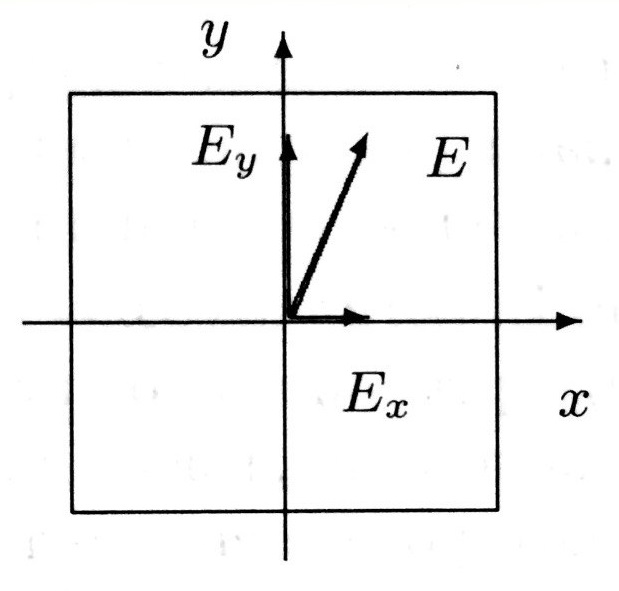
\includegraphics[width =  0.6\textwidth]{ris2}
			\caption{Разложение линейно поляризованного света по главным направлениям двоякопреломляющей пластинки.}
			\label{ris2}
		\end{figure}
	\end{minipage}\\

	 где $k$ -- волновое число для вакуума, d -- толщина кристаллической пластинки. Как уже отмечалось, при сложении двух взаимно перпендикулярных колебаний, обладающих некоторым сдвигом фаз, образуется колебание, поляризованное по эллипсу.
	 
	 \paragraph{Анализ эллиптически поляризованного света.} Анализ эллиптически поляризованного света сводится к нахождению главных осей эллипса поляризации и к определению направления вращения электрического вектора. 
	 
	 Главные оси эллипса поляризации определяются с помощью анализатора по максимуму и минимуму интенсивности проходящего света. Направление вращения электрического вектора может быть найдено с
	 помощью пластинки в четверть длины волны, для которой известно, какая из главных волн, $E_\xi$ или $E_\eta$, имеет большую скорость распространения (и, соответственно, меньшее значение показателя преломления).
	 
	 Выберем для определенности координатные оси $\xi$ и $\eta$ на пластинке так, чтобы
	 $n_\xi <
	 n_\eta$. В этом случае главная волна $E_\xi$ имеет большую скорость распространения. Поместим такую пластинку на пути эллиптически поляризованного света и совместим главные оси эллипса поляризации с главными направлениями пластинки $\lambda/4$. На выходе из этой пластинки сдвиг фаз между $E_\xi$ и $E_\eta$ вместо $\pi/2$ станет равным нулю или $\pi$. Свет окажется линейно поляризованным. Из двух возможных значе ний сдвига фаз, 0 или $\pi$, реализуется одно: то, которое соответствует имеющемуся в волне направлению вращения электрического вектора.
	 
	 Рассмотрим, например, случай, когда электрический вектор в эллиптически поляризованной волне вращается против часовой стрелки, если смотреть навстречу лучу. В этом случае, очевидно, в волне, падающей на пластинку в $\lambda/4$, колебание $E_\eta$ отстает по фазе на $ \pi/2$ от колебания $E_\xi$. При прохождении через пластинку разность фаз увеличивается до $\pi$. На выходе из пластинки, таким образом, возникают линейно поляризованные волны со сдвигом фаз $\pi$. Сложение этих волн дает плоско поляризованную волну, электрический вектор которой располагается во
	 втором и четвертом квадрантах координатной системы $\xi$, $\eta$.
	 
	 Рассуждая аналогичным образом, найдем, что при вращении электрического вектора по часовой стрелке направление колебаний в линейно поляризованной волне, выходящей из пластинки, располагается в первом и третьем квадрантах. Определяя направление колебаний на выходе из пластинки с помощью поляроида, можно, таким образом, определить характер эллиптической поляризации (вращение против или по часовой стрелке).
	 
	 \paragraph{Пластинка чувствительного оттенка.} Установить, какому из двух главных направления пластинки в четверть длины волны соответствует большая скорость распространения света, можно с помощью пластинки \textit{чувствительного оттенка} (так называют пластинку в $\lambda$ для зелёной спектрально компоненты, $\lambda = 560 ~ \text{нм}$).
	 
	 Пластинка имеет форму стрелы, вдоль оси которой расположено главное направление, соответствующее большей скорости распространения.
	 
	 Если пластинка чувствительного оттенка помещена между скрещенными поляроидами и главные направления пластинки не параллельны направлениям разрешённых колебаний поляроидов, то при освещении белым светом пластинка кажется окрашенной в лилово - красный цвет. Это объясняется тем, что зелёная компонента линейно поляризованного света при прохождении пластинки не меняет поляризации и задерживается вторым поляроидом. Для красной и фиолетовой компонент пластинка создаёт сдвиг фаз, несколько отличный от $2\pi$. На выходе из пластинки красная и фиолетовая компоненты оказываются поэтому эллиптически поляризованными и частично проходят через второй поляроид. Таким образом, в известном смысле наблюдаемый в указанном опыте цвет пластинки дополнителен к зелёному.
	 
	 Если между скрещенными поляроидами поместить пластинку чувствительного оттенка ($\lambda$) и пластинку в $\lambda/4$ так, чтобы их главные направления совпадали, цвет пластинки изменится. Если у пластинки чувствительного оттенка и пластинки в $\lambda /4$ совпадут главные направления, соответствующие большей скорости распространения, то разность хода между $E_x$ и $E_y$ для зелёного света составит уже $5\lambda/4$. Это соответствует разности хода в $\lambda$ для света с большей длиной волны, т.е. для <<более красного>> света. При освещении этих пластинок белым светом теперь погасится не зелёная, а красная часть спектра, и проходящий свет будет казаться зеленовато - голубым. Если же главные направления, соответствующие большей скорости распространения, у пластинки чувствительного оттенка и у пластинки в $\lambda / 4$ окажутся перпендикулярными, то проходящий свет приобретёт оранжево - жёлтую окраску (погасится фиолетово - голубая часть спектра).
	 
	 Изменение цвета позволяет, таким образом, определить какое из главных направлений пластинки в $\lambda / 4$ соответствует большей скорости.
	 
	 \paragraph{Интерференция поляризованных лучей.}
	 
	 Тонкие двоякопреломляющие пластинки, помещённые между поляроидами, кажутся окрашенными. Эта окраска может быть истолкована как результат интерференции поляризованных лучей. На рис. \ref{ris3} представлена схема для случая скрещенных поляроидов.
	 
	 \begin{minipage}{0.6\linewidth}
	 	Здесь $p_1 p'_1$ -- разрешённое направление колебаний первого поляроида; $x, y$ -- координатная система, связанная с главными направлениями двоякопреломляющей пластинки; $p_2 p'_2$ -- разрешённое направление колебаний второго поляроида. Волны $E_x$ и $E_y$ на выходе из пластинки когерентны, но не могут интерферировать, так как $E_x \bot E_y$. Волны $E_1$ и $E_2$ на выходе второго поляроида также являются когерентными и к тому же поляризованы в одной плоскости. Эти волны интерферируют между собой. Результат интерференции определяется зависящим от длины волны сдвигом фаз между $E_1$ и $E_2$. В результате интерференции поляризованных лучей пластинка, освещаемая белым светом, кажется окрашенной.
	 \end{minipage}
 	~
 	\begin{minipage}{0.3\linewidth}
 		\begin{figure}[H]
 			\centering
 			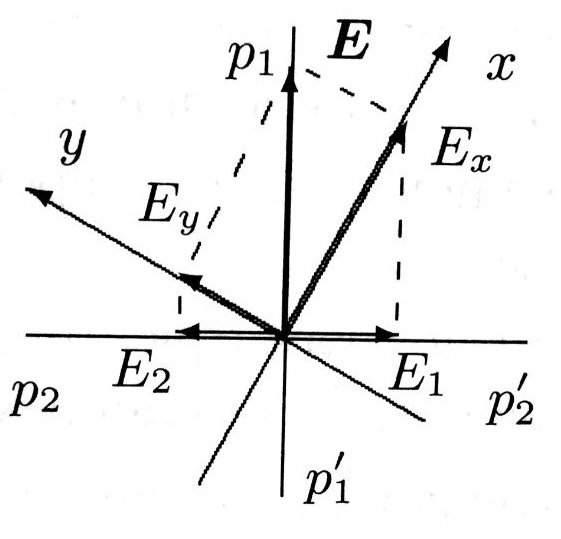
\includegraphics[width =  0.8\linewidth]{ris3}
 			\caption{К объяснению интерференции поляризованных лучей.}
 			\label{ris3}
 		\end{figure}
 	\end{minipage}
 
 Если поворачивать двоякопреломляющую пластинку, расположенную между скрещенными поляроидами, то соотношение амплитуд волн $E_1$ и $E_2$  и разность фаз между ними не изменяются. Это означает, что цвет пластинки при её поворотах не меняется, а меняется только интенсивность света. За один оборот пластинки интенсивность четыре раза обращается в нуль -- это происходит при совпадении главных направлений $x$ и $y$ с разрешёнными направлениями колебаний поляроидов.
 
 Если же двоякопреломляющую пластинку оставить неподвижной, а второй поляроид повернуть так, чтобы разрешённые направления $p_1 p'_1$ и $p_2 p'_2$ совпали, то волны $E_1$ и $E_2$ приобретают дополнительный фазовый сдвиг на $\pi$ для всех спектральных компонент; при этом их амплитуды изменяются так, что цвет пластинки изменится на дополнительный.
 
 
 \newpage
 	
	 
	 
	 
	 
	 \section{Ход работы.}
	
	\subsection{Определение разрешённых направлений поляроидов.}
	
	\begin{figure}[H]
		\centering
		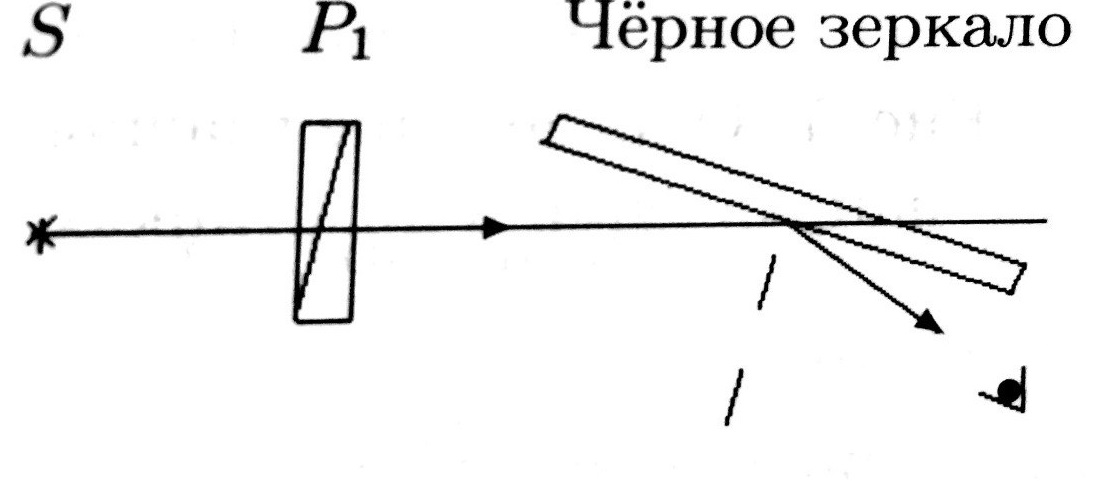
\includegraphics[width =  0.4\textwidth]{img1}
		\caption{Определение разрешённого направления поляроида.}
		\label{img1}
	\end{figure}

Соберём схему, показанную на рис. \ref{img1} для определения разрешенных направлений поляроидов.

Получим для 1 поляроида: разрешённое направление \textbf{горизонтально} при +10 \degree.

Разрешённое направление второго поляроида определим, скрестив поляроиды: после поляроида с известной поляризацией поставим второй поляроид и, глядя навстречу лучу, вращением второго поляроида добьёмся минимальной яркости луча.
	
Получим для 2 поляроида: разрешённое направление \textbf{вертикально} при -50 \degree.

\subsection{Определение угла Брюстера для эбонита.}

Поставим на скамью вместо чёрного зеркала эбонитовую пластину с круговой шкалой. Повернём эбонитовое зеркало вокруг вертикальной оси так, чтобы его плоскость была перпендикулярна лучу. Отметим начало отсчёта по лимбу: 270\degree.

Установим направление разрешённых колебаний поляроида $P_1$ горизонтально и найдём угол поворота эбонита $\varphi_\text{Б}$, при котором интенсивность отражённого луча минимальна: Конец отсчёта 325\degree.

Глаз не воспринимает изменение интенсивности при повороте на $\pm 3 \degree$.
Получаем, $$\varphi_\text{Б} = 55 \degree$$
$$n = \text{tg}\varphi_\text{Б} \Longrightarrow \fbox{$n \simeq 1.43 \pm 0.05 $}$$

Повторим изменения, добавив светофильтр Ф. В результате этого лишь уменьшилась интенсивность, а угол Брюстера не изменился.

\subsection{Исследование стопы.}

Поставим стопу стеклянных пластинок вместо эбонитового зеркала и подберём для нее такое положение, при котором свет падает на стопу под углом Брюстера. 

\begin{figure}[H]
	\centering
	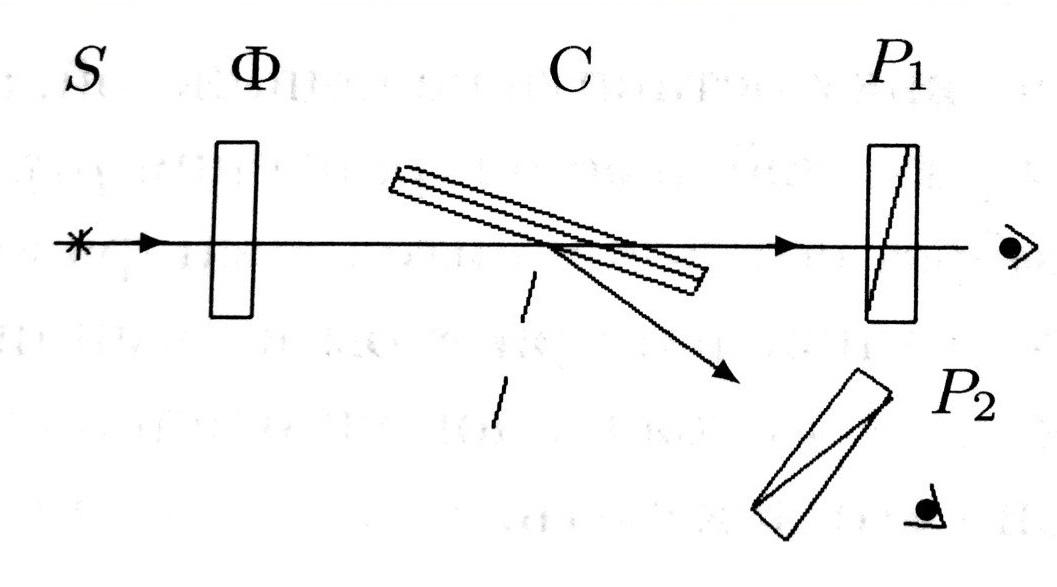
\includegraphics[width =  0.4\textwidth]{img2}
	\caption{Исследование стопы.}
	\label{img2}
\end{figure}

Осветим стопу неполяризованным светом и, рассматривая через поляроиды (рис \ref{img2}) свет, отражённый от стопы, определим ориентацию вектора $\mathbf{E}$ в отражённом луче: отражённый луч поляризован,\textit{ вектор $\mathbf{E}$ перпендикулярен плоскости падения}, т.е \textbf{вертикален}.

Преломлённый свет поляризован частично, максимальная интенсивность наблюдается при горизонтальном разрешённом направлении поляроида.

\subsection{Определение главных направлений двоякопреломляющих пластин.} 
	
	\begin{figure}[H]
		\centering
		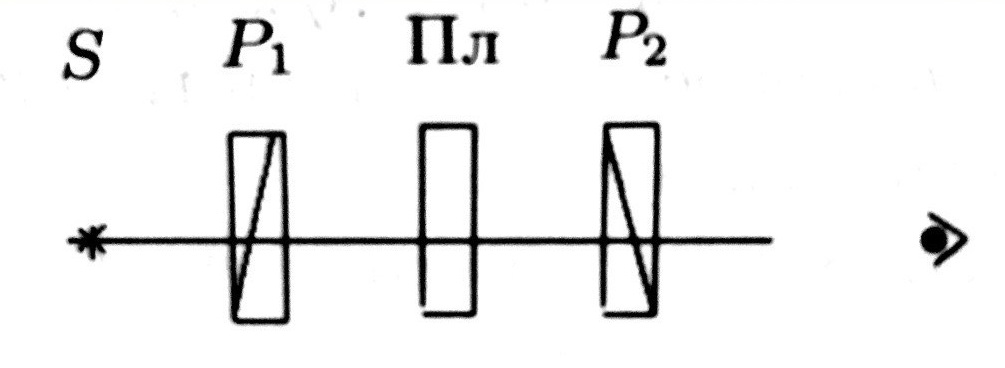
\includegraphics[width =  0.4\textwidth]{img3}
		\caption{Определение главных направлений в пластинках.}
		\label{img3}
	\end{figure}

Поставим кристаллическую пластинку между скрещенными поляроидами (рис. \ref{img3}). Вращая пластинку вокруг направления луча и наблюдая за интенсивностью света, найдём положение пластинки, при котором интенсивность минимальна. В таком положении разрешённые направления поляроидов совпадают с главными направлениями пластин.

Для чёрной пластины: \textit{min} при 260 \degree.

Для серебристой пластины: \textit{min} при 50 \degree.

\subsection{Выделение пластин $\frac{\lambda}{2}$ и $\frac{\lambda}{4}$.}

Добавим к схеме изображённой на рис.\ref{img3} зелёный фильтр. Установим разрешённое направление первого поляроида горизонтально, а главные направления исследуемой пластинки -- под углом 45 \degree к горизонтали.

Получаем, что в опыте с серебристой пластиной интенсивность света при вращении 2 поляроида практически не меняется $\Rightarrow$ поляризация круговая $\Rightarrow$ 
\begin{center}
	\fbox{
серебристая пластинка -- $\lambda/4$}	
\end{center}

В опыте с чёрной пластинкой интенсивность имеет ярко выраженный максимум и минимум $\Rightarrow$ линейная поляризация $\Rightarrow$

\begin{center}
	\fbox{
	чёрная пластинка -- $\lambda/2$}
\end{center}

\subsection{Определение направлений <<быстрой>> и <<медленной>> оси в пластинке $\lambda/4$.}

\begin{figure}[H]
	\centering
	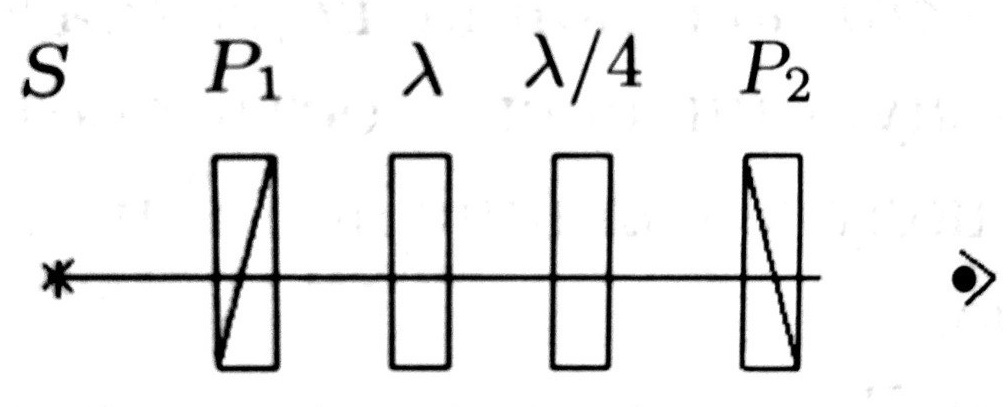
\includegraphics[width =  0.4\textwidth]{img4}
	\caption{Определение направлений большей и меньшей скорости.}
	\label{img4}
\end{figure}

Поставим между скрещенными поляроидами пластинку чувствительного оттенка ($\lambda$ для зелёного цвета), имеющую вид стрелки. Световой вектор, ориентированный вдоль направления стрелки, проходит с большей скоростью, перпендикулярный с меньшей.

Добавим к схеме пластинку $\lambda/4$ (рис.\ref{img4}), главные направления которой совпадают с главными направлениями пластины $\lambda$ и ориентированы под углом 45 \degree к разрешённым направлениям скрещенных поляроидов.

При вращении пластинки относительно пластинки чувствительного оттенка цвет стрелки менялся от голубого до жёлтого. В положении, когда цвет голубой, быстрые направления пластинок совпадают, когда жёлтый, они перпендикулярны.

Получаем, что \textit{быстрая ось вертикальна при 135 \degree.}

\subsection{Интерференция поляризованных лучей.}

Расположим между скрещенными поляроидами мозаичную слюдяную пластинку. Она собрана из 4-х узких полосок слюды, лежащих по сторонам квадрата (дву полоски <<толщиной>> $\lambda/4$ и по одной -- $\lambda/2$ и $3\lambda/4$). В центральном квадратике слюды нет. Главные направления всех пластинок ориентированы параллельно сторонам квадрата.

При вращении мозаичной пластинки менялась только интенсивность света, а цвета оставались неизменными. За один оборот пластинки интенсивность четыре раза обращается в нул -- это происходит при совпадении главных направлений $x$ и $y$ с разрешёнными направлениями колебаний поляроидов.

Вращая 2 поляроид, мы заметили, что менялись цвета квадрантов. Это происходило в том случае, когда направления $p_1p'_1$ и $p_2p'_2$ совпадали (см рис. \ref{ris3}). В этом случае волны $E_1$ и $E_2$ приобретают дополнительный фазовый сдвиг на $\pi$ для всех спектральных компонент (то есть, те спектральные линии, которые имели максимум, теперь имеют минимум) $\Rightarrow$ цвет пластинки изменяется на дополнительный.

\subsection{Определение направления вращения светового вектора в эллиптически поляризованной волне. }

\begin{enumerate}
	\item Нарисуем эллипс поляризации для вектора $\mathbf{E}$, вышедшего из пластинки $\lambda/4$, и укажем на нём направление большей и меньшей скорости. Рядом нарисуем две вышедших из пластинки синусоиды: $x(t)$ и $y(t)$ со сдвигом фаз в четверть периода (рис. \ref{ris4}).
	
	Пусть $x$ -- направление быстрой оси, то $E_x$ опережает по фазе на $T/4$ $E_y$. 
	
	\begin{figure}[H]
		\centering
		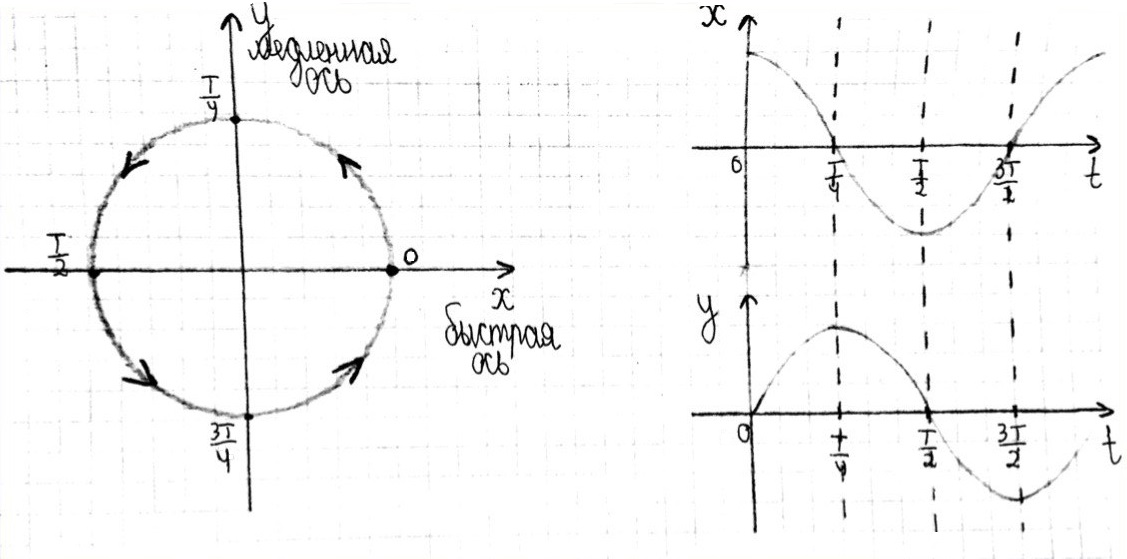
\includegraphics[width =  0.7\linewidth]{ris4}
		\caption{К определению направления эллиптической поляризации.}
		\label{ris4}
	\end{figure} 

	\item Получим эллиптически-поляризованный свет. Для этого установим разрешённое направление первого поляроида под углом 30 \degree к горизонтали так, чтобы вектор $\mathbf{E}$ падающего на пластинку света был расположен в первом квадранте. Установим разрешённое направление второго поляроида вертикально и, вращая пластинку найдём минимальную интенсивность света, прошедшего второй поляроид. Вращая второй поляроид, убедимся что свет поляризован эллиптически, а не линейно. Таким образом, мы получили эллипс поляризации с вертикально ориентированной малой осью.
	
	\item Для определения направления вращения светового вектора в эллипсе установим между поляроидами дополнительную пластинку $\lambda /4$ с известными направлениями <<быстрой>> и <<медленной>> осей, ориентированными по осям эллипса поляризации анализируемого света. В этом случае вектор $\mathbf{E}$ на выходе будет таким, как если бы свет прошел две пластинки $\lambda /4$: свет на выходе из второй пластинки будет линейно поляризован. 
	
	Получаем, что световой вектор перешел в смежные квадранты (на выходе из 1 поляризатора он лежит в 1 и 3 квадрантах, а после прохождения пластинок во 2 и 4 квадрантах). Значит, разность фаз, даваемая пластинками не скомпенсировалась, а сложилась. Значит, эллипсы вращаются в одну сторону.
	
	Из пункта 1 получаем, что эллипсы поляризации ориентированы \begin{center}
	\fbox{против часовой стрелки}.	
	\end{center}
\end{enumerate}

\section{Вывод.}
В результате проведения этой лабораторной работы, мы 
\begin{itemize}
	\item ознакомились с методами получения и анализа поляризованного света.
	
	\item исследовали явление интерференции поляризованного света.
	
	\item измерили коэффициент преломления эбонита.
	
	\item определили направление вращения вектора $E$ эллиптически поляризованного света.
\end{itemize}

\end{document}